% !TEX root = bmc_microbiology_curli_vagal_pd_manuscript.tex
\documentclass[12pt]{article}
\usepackage[margin=1in]{geometry}
\usepackage{amsmath}
\usepackage{booktabs}
\usepackage{longtable}
\usepackage{graphicx}
\usepackage{float}
\usepackage{placeins}
\usepackage{hyperref}
\usepackage{authblk}
\usepackage{setspace}
\usepackage{natbib}
\doublespacing

\title{Cross-cohort evidence synthesis identifies recurrent elevation of curli-carrier bacterial burden in Parkinson's disease gut metagenomes}
\author[1]{Nabanita Ghosh}
\author[2]{Krishnendu Sinha}
\affil[1]{Department of Zoology, Maulanan Azad College, Kolkata, India}
\affil[2]{Department of Zoology, Jhargram Raj College, Jhargram, India}
\date{}

\emergencystretch=3em
\sloppy
\begin{document}
\maketitle

\noindent\textbf{Running title:} Curli Carrier Burden in Parkinson's disease gut metagenomes\\
\textbf{Corresponding author:} Nabanita Ghosh, nabanitaghosh89@gmail.com\\
\textbf{Keywords:} Parkinson's disease; gut microbiome; curli amyloid; bacterial amyloid; metagenomics; Enterobacteriaceae; Curli Carrier Burden; gut-brain axis

\section*{Abstract}
\subsection*{Background}
Parkinson's disease (PD) is associated with reproducible gut microbiome alterations, but biologically informed summaries of amyloidogenic bacterial taxa remain underdeveloped. Curli is a bacterial amyloid produced by several Enterobacteriaceae and related organisms, making curli-carrier taxa a plausible microbial feature for gut-brain-axis studies involving host amyloid biology and immune signaling. We introduced Curli Carrier Burden (CCB), a reproducible taxon-informed computational index that quantifies the aggregate abundance of curli-carrier bacterial taxa in processed gut metagenomic profiles.

\subsection*{Results}
We applied the CCB framework to public processed PD gut metagenomic cohorts spanning Wallen discovery, Integrated-US replication, Mao Central China replication, and Romano non-Wallen multi-study analysis. Wallen showed a discovery-stage PD-enriched signal. Integrated-US provided statistically supported independent replication, with higher PD CCB by Mann--Whitney testing and significant adjusted burden and presence models. Mao Central China showed the same PD-greater-than-control direction by mean and median CCB. Romano non-Wallen analysis included 600 samples from 6 studies and showed higher PD than HC CCB by mean and median, with a pooled Mann--Whitney $p=0.0036$ and Cliff's delta 0.137; study-stratified permutation testing was cohort-sensitive ($p=0.1974$).

\subsection*{Conclusions}
CCB identifies recurrent PD-associated elevation of curli-carrier bacterial burden across processed public gut metagenomic cohorts. The findings support a reproducible computational framework for microbiology-focused PD microbiome analysis and motivate future raw-read, gene-centric, and strain-resolved validation of curli biology in PD-associated gut microbial communities.

\section*{Background}
Parkinson's disease is increasingly studied as a systemic disorder with prominent gastrointestinal and microbial dimensions. Public gut metagenomic studies have reported taxonomic differences between PD and control participants, supporting a role for microbial community structure in disease-associated gut ecology \citep{Romano2021NPJPD,Wallen2022NatCommun}. A microbiology-first interpretation of these studies requires methods that move beyond individual taxa and summarize microbial traits with plausible host relevance.

Bacterial amyloids provide one such trait class. Curli fibres are extracellular amyloid structures produced by several Enterobacteriaceae and related taxa, and have been discussed in relation to host amyloid biology, immune activation, epithelial barrier effects, and alpha-synuclein-centered gut-brain-axis hypotheses \citep{Barnhart2006Curli,Chen2016CurliAlphaSyn}. Existing PD microbiome analyses commonly report species-level or genus-level shifts, but they do not directly summarize the aggregate burden of curli-carrier bacterial taxa.

Here we introduce Curli Carrier Burden (CCB), a biologically informed computational index designed for processed metagenomic profiles. CCB quantifies the abundance of curated curli-carrier taxa while preserving a conservative interpretation as a taxon-informed proxy rather than direct measurement of curli genes or expression. We developed and applied this framework across public processed PD gut metagenomic cohorts, using Wallen as discovery evidence and Integrated-US, Mao Central China, and Romano non-Wallen analyses as external evidence streams.

\section*{Methods}
\subsection*{Study design}
This study was a computational cross-cohort evidence synthesis of public processed gut metagenomic datasets. The analysis evaluated whether CCB, an aggregate abundance index of curli-carrier taxa, showed recurrent elevation in PD relative to controls across independent processed metagenomic cohorts.

\subsection*{Public processed metagenomic cohorts}
The synthesis used four analyzed datasets: Wallen discovery, Integrated-US multicohort replication, Mao Central China replication, and Romano non-Wallen multi-study replication. Wallen was treated as discovery evidence and was not counted as independent replication. Integrated-US was treated as the primary independent replication cohort. Mao Central China was treated as an external processed-table replication cohort. Romano non-Wallen was treated as a multi-study external replication analysis with explicit cohort-aware robustness evaluation. Dataset-level summaries are shown in Table~\ref{tab:datasets}.

\subsection*{Curli-carrier taxon curation}
Curli-carrier candidate taxa were curated from project Phase 1 reference outputs and matched to processed abundance profiles using exact species and binomial species-level matching where possible. Genus-level fallback matches were retained only for transparency and exploratory interpretation, not as primary burden taxa. Candidate matching files and burden species sets were preserved for each analyzed cohort.

\subsection*{Curli Carrier Burden index}
For sample $s$, Curli Carrier Burden was defined as
\[
\mathrm{CCB}_{s} = \sum_{i=1}^{m} a_{is} w_i
\]
where $a_{is}$ is the relative abundance of curli-carrier taxon $i$ in sample $s$, $w_i$ is the evidence or confidence weight assigned to taxon $i$, and $m$ is the number of matched curli-carrier taxa in the abundance profile. The confidence weights were defined as
\[
w_i =
\begin{cases}
1.00, & \text{high-confidence curli-carrier taxon} \\
0.50, & \text{medium-confidence curli-carrier taxon} \\
0.25, & \text{low-confidence curli-carrier taxon}.
\end{cases}
\]
CCB is a taxon-informed proxy of curli-carrier bacterial burden in processed metagenomic profiles, not a direct measurement of \textit{csg} gene abundance, operon integrity, or curli expression. Logistic regression models used a transformed burden where appropriate:
\[
\log(1 + \mathrm{CCB}_{s}).
\]

\subsection*{Dataset-specific analyses}
Each cohort was analyzed using its validated processed species or taxonomic abundance table and corresponding phenotype metadata. Sample identifiers were required to match between metadata and abundance matrices. PD and control labels were mapped according to dataset-specific validated rules documented in the project reports.

\subsection*{Wallen discovery analysis}
The Wallen discovery analysis included 724 samples, comprising 490 PD and 234 controls. Curli-carrier taxa were matched to the processed abundance table, CCB was computed for each sample, and PD-control comparisons used non-parametric testing and logistic regression models.

\subsection*{Integrated-US replication analysis}
The Integrated-US replication analysis included 244 samples, comprising 95 PD and 149 controls. The primary outcome was PD status, and the primary predictor was $\log(1+\mathrm{CCB})$. Secondary analyses evaluated curli-carrier presence. Sensitivity analyses compared PD separately against spouse/partner controls and healthy controls where available.

\subsection*{Mao Central China replication analysis}
The Mao Central China analysis included 78 samples, comprising 39 PD and 39 spouse controls. Because curli-carrier presence lacked variation in this cohort, presence-based logistic modeling was considered non-informative. The primary burden analysis used Mann--Whitney testing and unadjusted burden logistic regression, with a paired spouse-control sensitivity analysis when pair identifiers were inferable.

\subsection*{Romano non-Wallen replication analysis}
The Romano non-Wallen analysis used processed mOTUs profiles and excluded Wallen-derived samples. The final analysis set was Romano\_nonWallen\_600, comprising 600 samples, 280 PD, 320 HC, and 6 studies. The CCB candidate source was the curated Phase 1/2B curli candidate table. A total of 29 curli-associated mOTUs taxa were matched.

\subsection*{Cross-cohort evidence synthesis}
Phase 2P synthesized cohort-level evidence from Wallen, Integrated-US, Mao Central China, and Romano non-Wallen reports. For each dataset, the synthesis captured sample counts, matched taxa, PD and control CCB means and medians, primary $p$ values, cohort-aware or study-aware $p$ values where available, effect sizes, robustness summaries, and final evidence tiers.

\subsection*{Statistical analysis}
Cohort-specific statistical tests used Mann--Whitney U tests for non-parametric PD-control burden comparisons and logistic regression for PD status where the input data supported regression modeling. Logistic models reported coefficients, odds ratios, Wald confidence intervals, nominal $p$ values, and Benjamini--Hochberg adjusted $q$ values where implemented in prior phase outputs. Romano included pooled Mann--Whitney testing, Cliff's delta, and study-stratified permutation testing.

\subsection*{Robustness and cohort-aware analyses}
Robustness analyses included sensitivity models in Integrated-US, paired or spouse-control sensitivity in Mao, leave-one-study-out analyses in Romano, and within-study Romano effect summaries. These analyses were used to distinguish recurrent directionality from cohort-sensitive statistical support.

\subsection*{Reproducibility}
All analyses used existing public processed metagenomic profiles and project scripts archived in the repository. Phase-specific outputs were written as tab-separated files and plain-text reports. The Phase 2P evidence synthesis used only existing report files and did not download data, process raw reads, or perform new metagenomic profiling.

\subsection*{Ethics statement}
This study used publicly available, de-identified processed metagenomic datasets and did not involve new human participant recruitment or new sample collection.

\section*{Results}
\subsection*{Curli Carrier Burden framework and curated curli-carrier taxa}
We developed CCB as a reproducible taxon-informed measure of aggregate curli-carrier bacterial burden in processed metagenomic profiles. Across datasets, the primary burden calculation used species-level or binomial taxon matches when available. This strategy prioritizes microbiological specificity while retaining transparent documentation of candidate matching.

\subsection*{Wallen discovery analysis}
In Wallen, CCB was higher in PD than controls by both mean and median values. The discovery analysis included 724 samples and 31 matched curli-carrier taxa. PD mean and median CCB were 1.81 and 0.0682, compared with control mean and median values of 1.39 and 0.0194. The primary burden comparison was significant ($p=0.002$), establishing discovery-stage PD enrichment.

\subsection*{Integrated-US replication analysis}
Integrated-US provided supportive independent replication. The analysis included 244 samples, 95 PD and 149 controls, with 18 primary burden species. PD mean and median CCB exceeded control values (2/0.125 versus 1.82/0). The primary Mann--Whitney comparison was significant ($p=0.0079$), and the adjusted log-transformed burden model supported replication.

\subsection*{Mao Central China replication analysis}
Mao Central China showed directionally consistent CCB elevation in PD. The analysis included 78 samples, balanced between 39 PD and 39 controls, with 17 burden species. PD mean and median CCB were 6.88 and 2.08, compared with control values of 4.56 and 1.71. The primary test was not statistically significant ($p=0.2673$), but the direction was consistent with Wallen and Integrated-US.

\subsection*{Romano non-Wallen replication analysis}
Romano non-Wallen analysis provided a large multi-study external evidence stream. The analysis set Romano\_nonWallen\_600 included 600 samples (280 PD and 320 HC) from 6 studies, with 29 matched curli-associated mOTUs taxa. PD median CCB was 9.72e-04, compared with HC median CCB of 5.97e-04. PD mean CCB was 0.0153, compared with HC mean CCB of 0.0104. The pooled Mann--Whitney test was significant ($p=0.0036$), with Cliff's delta 0.137.

\subsection*{Romano cohort-aware robustness}
Romano robustness analyses supported a cohort-aware interpretation. Leave-one-study-out analyses retained PD-greater-than-HC direction by both mean and median CCB. Within-study analyses showed PD-greater-than-HC direction by mean in 4 of 6 studies and by median in 3 of 6 studies, with nominal $p<0.05$ in 2 of 6 studies. The study-stratified permutation test was not significant ($p=0.1974$), indicating that Romano provides directionally supportive but cohort-sensitive evidence rather than definitive replication.

\subsection*{Cross-cohort evidence synthesis}
The Phase 2P synthesis included Wallen discovery, Integrated-US replication, Mao Central China replication, and Romano non-Wallen replication (Table~\ref{tab:cross-cohort-evidence}). All four analyzed datasets showed PD-greater-than-control direction by mean and median CCB. Integrated-US provided supportive statistically significant independent replication, Mao provided directionally consistent evidence, and Romano provided directionally supportive cohort-sensitive evidence. Together, these analyses identified a recurrent PD-associated elevation of CCB across processed public metagenomic cohorts, while highlighting the value of cohort-aware interpretation.


\FloatBarrier

\begin{figure}[H]
\centering
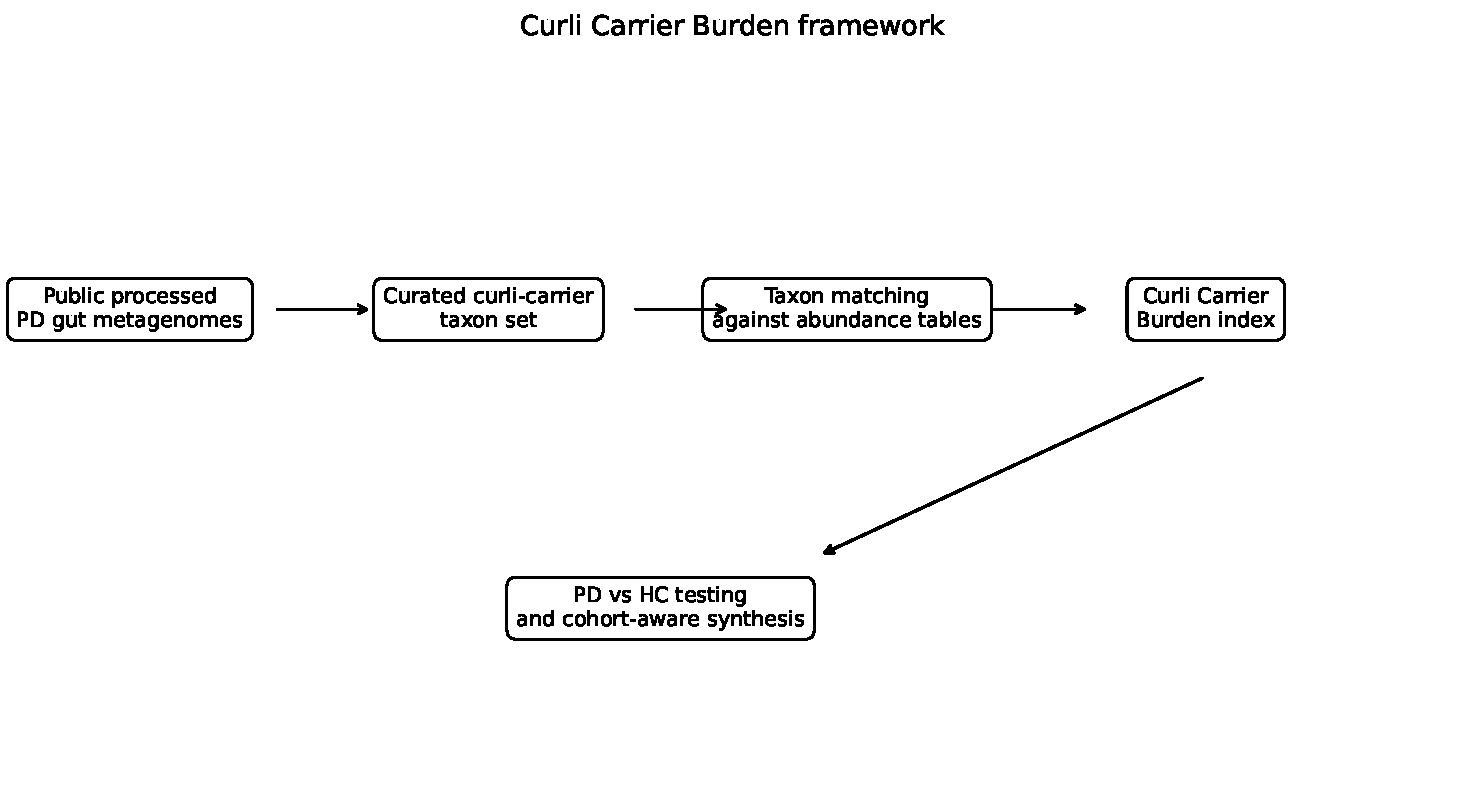
\includegraphics[width=0.95\textwidth]{figures/figure1_ccb_workflow.pdf}
\caption{\textbf{Workflow of the Curli Carrier Burden framework.} Public processed Parkinson's disease gut metagenomic profiles were integrated with a curated curli-carrier taxon set. Matched taxa were used to compute sample-wise Curli Carrier Burden, followed by PD--HC comparison and cross-cohort evidence synthesis.}
\label{fig:ccb-workflow}
\end{figure}

\begin{figure}[H]
\centering
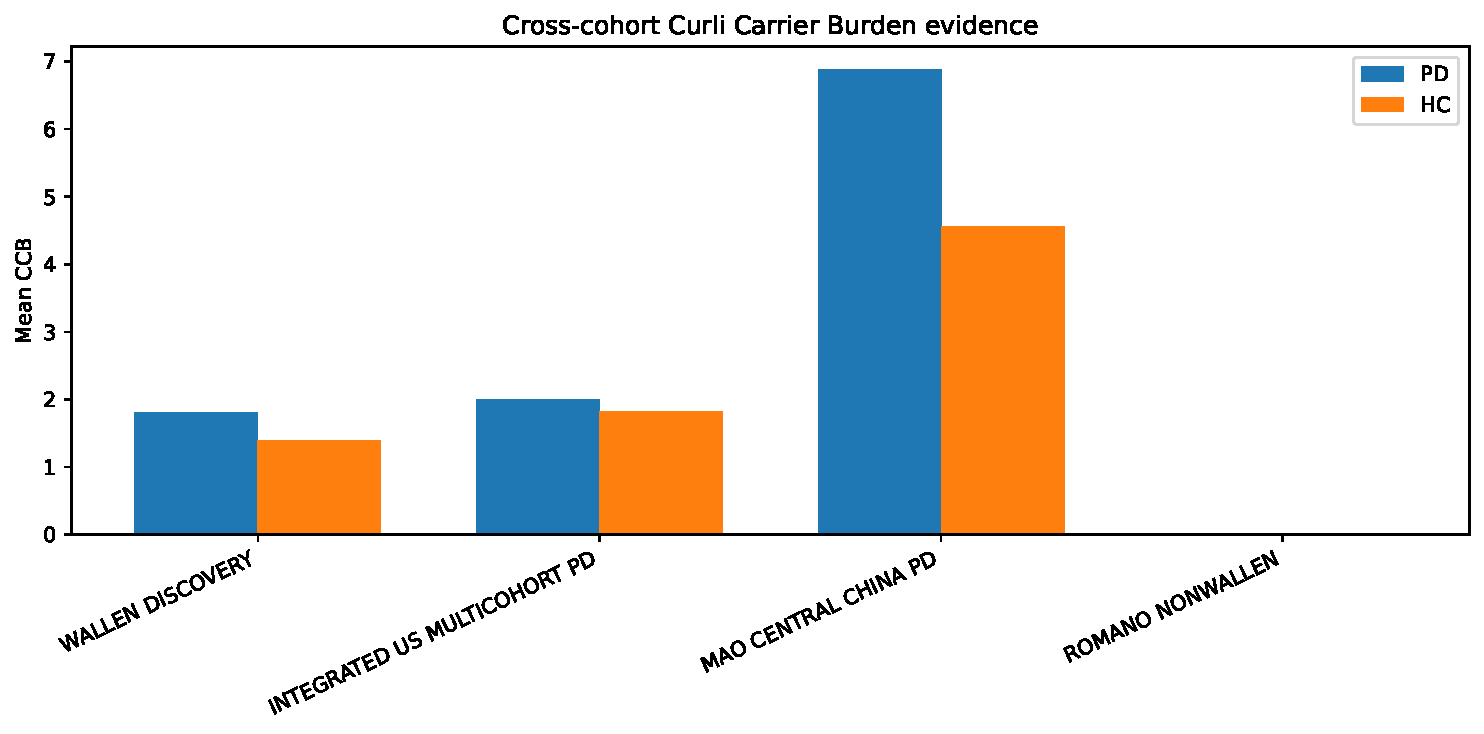
\includegraphics[width=0.95\textwidth]{figures/figure2_cross_cohort_ccb.pdf}
\caption{\textbf{Cross-cohort Curli Carrier Burden evidence across processed public PD gut metagenomic cohorts.} The figure summarizes mean Curli Carrier Burden in PD and control groups across the analyzed discovery and replication datasets using a log-scaled y-axis to display cohort-specific abundance scales.}
\label{fig:cross-cohort-ccb}
\end{figure}

\begin{figure}[H]
\centering
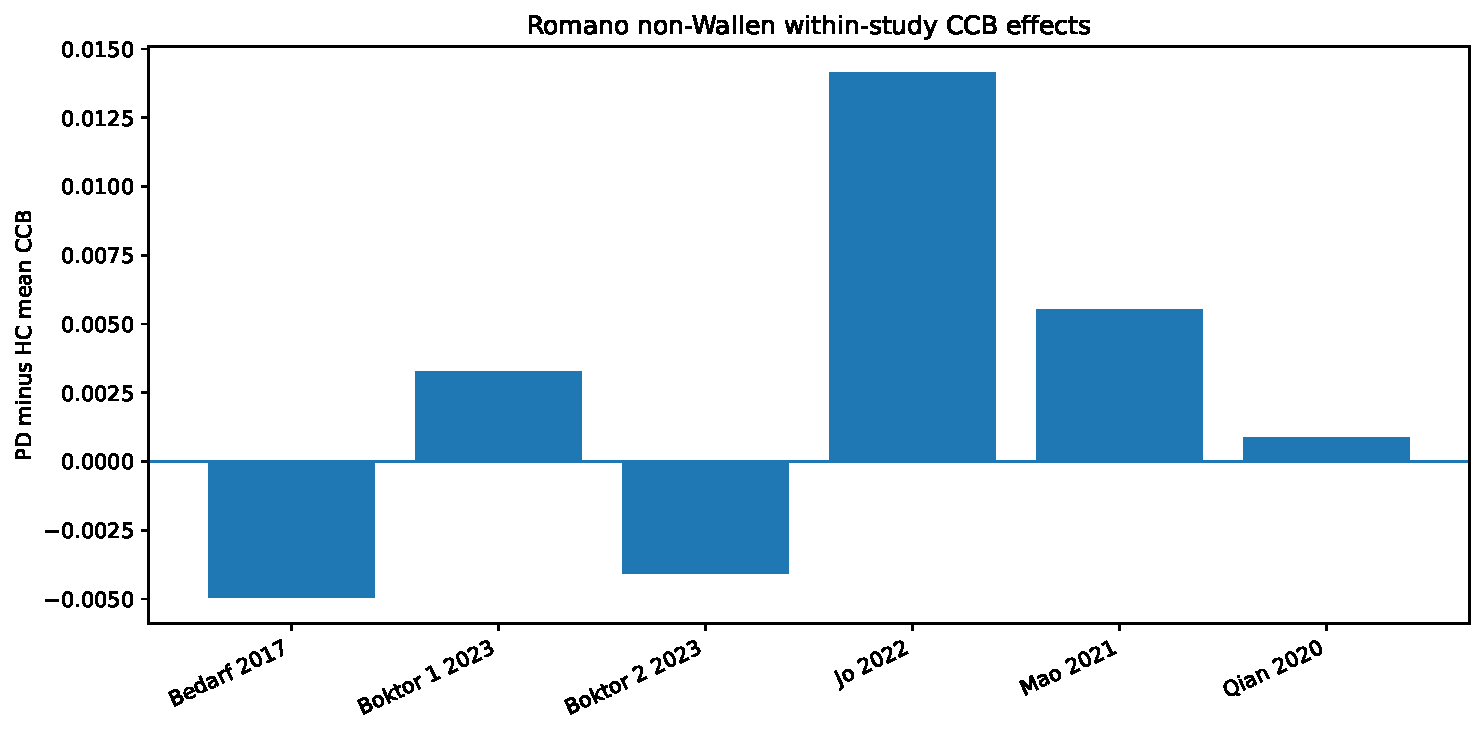
\includegraphics[width=0.95\textwidth]{figures/figure3_romano_within_study.pdf}
\caption{\textbf{Romano non-Wallen within-study Curli Carrier Burden effects.} Bars show the mean PD-minus-control Curli Carrier Burden difference within each non-Wallen Romano study subset, illustrating cohort-aware interpretation of the Romano replication analysis.}
\label{fig:romano-within-study}
\end{figure}

\FloatBarrier

\section*{Discussion}
This study introduces CCB as a novel microbiology-informed index for quantifying curli-carrier bacterial burden in processed gut metagenomic profiles. By aggregating curated curli-carrier taxa into a reproducible burden measure, CCB translates a mechanistically plausible bacterial trait into a cohort-level microbiome feature that can be compared across public datasets.

The cross-cohort evidence supports recurrent PD-associated elevation of CCB. Wallen established discovery evidence, Integrated-US provided statistically supported independent replication, Mao Central China showed the same direction of effect, and Romano non-Wallen added a large multi-study analysis with directionally supportive but cohort-sensitive robustness. This pattern is compatible with gut-brain-axis hypotheses involving bacterial amyloids, immune activation, barrier biology, and alpha-synuclein-related host responses.

Romano should be interpreted as an informative multi-study analysis rather than a negative result. The pooled Romano analysis was directionally supportive and statistically significant, while study-stratified testing emphasized cohort heterogeneity. This strengthens interpretation by showing that CCB should be evaluated with cohort-aware methods rather than treated as a uniform effect across all public profiles.

The CCB framework is reusable. The same approach can be applied to additional PD cohorts, strain-resolved profiles, gene-centric abundance tables, and other amyloidogenic or immune-relevant microbial traits. Because the index is defined mathematically and implemented from explicit taxon matching rules, it supports transparent extension as new curli biology and microbial reference annotations become available.

Because this study used processed public metagenomic profiles, CCB represents a taxon-informed estimate of curli-carrier burden rather than direct \textit{csg} operon quantification; future raw-read and gene-centric analyses will be valuable for validating gene-level curli abundance and strain-level contributions.

\section*{Conclusions}
We introduced Curli Carrier Burden as a reproducible index of amyloidogenic curli-carrier bacterial burden in processed gut metagenomic profiles. Across Wallen, Integrated-US, Mao Central China, and Romano non-Wallen analyses, CCB showed recurrent PD-associated elevation, with statistically supported independent replication in Integrated-US and directionally supportive external evidence in Mao and Romano. These results support future gene-centric, raw-read, strain-resolved, and prospective validation of curli-carrier bacterial ecology in PD gut microbiome research.

\section*{Declarations}
\subsection*{Ethics approval and consent to participate}
This study used publicly available, de-identified processed metagenomic datasets and did not involve new human participant recruitment or new sample collection.

\subsection*{Consent for publication}
Not applicable.

\subsection*{Availability of data and materials}
The analysis used public processed metagenomic datasets and derived project reports. Repository accession, dataset source, and code availability details will be completed before submission. The analysis code and generated summary tables will be made available through a public repository or archive.

\subsection*{Competing interests}
The authors declare that they have no competing interests.

\subsection*{Funding}
No specific funding was received for this study.

\subsection*{Authors' contributions}
Author contributions will be finalized after confirmation of the complete author list.

\subsection*{Acknowledgements}
The authors acknowledge the investigators who generated and released the public Parkinson's disease gut metagenomic datasets analyzed in this study.

\begin{table}
\centering
\scriptsize
\setlength{\tabcolsep}{3pt}[htbp]
\centering
\caption{Public processed gut metagenomic cohorts included in the Curli Carrier Burden evidence synthesis.}
\label{tab:datasets}
\small
\resizebox{\textwidth}{!}{%
\begin{tabular}{llllrrl}
\hline
Dataset & Role & Source type & $n$ & PD & Control & Analysis use \\
\hline
Wallen & Discovery & Processed public gut metagenomic abundance profiles & 724 & 490 & 234 & Discovery PD Enriched Signal \\
Integrated-US & Independent replication & Processed public gut metagenomic abundance profiles & 244 & 95 & 149 & Replicated Directionally And Statistically \\
Mao Central China & External replication & Processed public gut metagenomic abundance profiles & 78 & 39 & 39 & Directionally Consistent But Not Significant \\
Romano non-Wallen & External replication, non-Wallen & Processed public mOTUs profiles, non-Wallen subset & 600 & 280 & 320 & Weak Cohort Sensitive Support Not Definitive Replication \\
\hline
\end{tabular}
}
\end{table}

\begin{table}
\centering
\scriptsize
\setlength{\tabcolsep}{3pt}[htbp]
\centering
\caption{Cross-cohort evidence for PD-associated elevation of Curli Carrier Burden (CCB).}
\label{tab:cross-cohort-evidence}
\small
\resizebox{\textwidth}{!}{%
\begin{tabular}{lllrrrrll}
\hline
Dataset & Role & $n$ & Matched taxa & PD mean/median & Control mean/median & Primary $p$ & Cohort-aware $p$ & Evidence decision \\
\hline
Wallen & Discovery & 724 & 31 & 1.81/0.0682 & 1.39/0.0194 & 0.002 & not available & Discovery PD Enriched Signal \\
Integrated-US & Independent replication & 244 & 18 & 2/0.125 & 1.82/0 & 0.0079 & not available & Replicated Directionally And Statistically \\
Mao Central China & External replication & 78 & 17 & 6.88/2.08 & 4.56/1.71 & 0.2673 & not available & Directionally Consistent But Not Significant \\
Romano non-Wallen & External replication, non-Wallen & 600 & 29 & 0.0153/9.72e-04 & 0.0104/5.97e-04 & 0.0036 & 0.1974 & Weak Cohort Sensitive Support Not Definitive Replication \\
\hline
\end{tabular}
}
\end{table}

\begin{table}[htbp]
\centering
\caption{Romano non-Wallen robustness analyses showing cohort-aware interpretation of Curli Carrier Burden.}
\label{tab:romano-robustness}
\small
\begin{tabular}{lrrrlll}
\hline
Condition & $n$ & PD & HC & Mean direction & Median direction & $p$ value \\
\hline
Full Romano non-Wallen set & 600 & 280 & 320 & PD>HC & PD>HC & 0.0036 \\
Leave out Bedarf\_2017 & 541 & 249 & 292 & PD>HC & PD>HC & 2.89e-04 \\
Leave out Boktor\_1\_2023 & 487 & 234 & 253 & PD>HC & PD>HC & 0.1148 \\
Leave out Boktor\_2\_2023 & 486 & 238 & 248 & PD>HC & PD>HC & 0.005 \\
Leave out Jo\_2022 & 444 & 198 & 246 & PD>HC & PD>HC & 0.0776 \\
Leave out Mao\_2021 & 522 & 241 & 281 & PD>HC & PD>HC & 0.0106 \\
Leave out Qian\_2020 & 520 & 240 & 280 & PD>HC & PD>HC & 6.59e-04 \\
\hline
\multicolumn{7}{l}{\textit{Within-study summaries}} \\
\hline
Bedarf\_2017 & 59 & 31 & 28 & PD<=HC & PD<=HC & 0.1161 \\
Boktor\_1\_2023 & 113 & 46 & 67 & PD>HC & PD>HC & 0.0073 \\
Boktor\_2\_2023 & 114 & 42 & 72 & PD<=HC & PD>HC & 0.2455 \\
Jo\_2022 & 156 & 82 & 74 & PD>HC & PD>HC & 0.0089 \\
Mao\_2021 & 78 & 39 & 39 & PD>HC & PD<=HC & 0.2716 \\
Qian\_2020 & 80 & 40 & 40 & PD>HC & PD<=HC & 0.3383 \\
\hline
\end{tabular}
\end{table}




\begin{thebibliography}{99}

\bibitem[Romano et~al.(2021)]{Romano2021NPJPD}
Romano S, Savva GM, Bedarf JR, Charles IG, Hildebrand F, Narbad A.
Meta-analysis of the Parkinson's disease gut microbiome suggests alterations linked to intestinal inflammation.
\textit{npj Parkinson's Disease}. 2021;7:27. doi:10.1038/s41531-021-00156-z.

\bibitem[Wallen et~al.(2022)]{Wallen2022NatCommun}
Wallen ZD, Appah M, Dean MN, Sesler CL, Factor SA, Molho E, Zabetian CP, Standaert DG, Payami H.
Metagenomics of Parkinson's disease implicates the gut microbiome in multiple disease mechanisms.
\textit{Nature Communications}. 2022;13:6958. doi:10.1038/s41467-022-34667-x.

\bibitem[Barnhart and Chapman(2006)]{Barnhart2006Curli}
Barnhart MM, Chapman MR.
Curli biogenesis and function.
\textit{Annual Review of Microbiology}. 2006;60:131--147. doi:10.1146/annurev.micro.60.080805.142106.

\bibitem[Chen et~al.(2016)]{Chen2016CurliAlphaSyn}
Chen SG, Stribinskis V, Rane MJ, Demuth DR, Gozal E, Roberts AM, Jagadapillai R, Liu R, Choe KY, Shivakumar B, Son F, Jin S, Kerber R, Adame A, Masliah E, Friedland RP.
Exposure to the functional bacterial amyloid protein curli enhances alpha-synuclein aggregation in aged Fischer 344 rats and \textit{Caenorhabditis elegans}.
\textit{Scientific Reports}. 2016;6:34477. doi:10.1038/srep34477.

\bibitem[Mao et~al.(2021)]{Mao2021FrontMicrobiol}
Mao L, Zhang Q, Li H, Chen Y, Li Y, Huang X, Zheng P, Li J, Li X, Chen J, Xie P.
Cross-sectional study on the gut microbiome of Parkinson's disease patients in central China.
\textit{Frontiers in Microbiology}. 2021;12:728479. doi:10.3389/fmicb.2021.728479.

\bibitem[Boktor et~al.(2023)]{Boktor2023MovDisord}
Boktor JC, Sharon G, Verhagen Metman LA, Lee SJ, Matheoud D, Sampson TR, Gradinaru V.
Integrated multi-cohort analysis of the Parkinson's disease gut metagenome.
\textit{Movement Disorders}. 2023;38:399--409. doi:10.1002/mds.29300.

\bibitem[Qian et~al.(2020)]{Qian2020Brain}
Qian Y, Yang X, Xu S, Huang P, Li B, Du J, He Y, Su B, Xu L, Wu B, Wang L, Liu M, Chen S, Wang X, Jin H, Zhang L, Li H, Zhang Y, Liu J, Wang H.
Gut metagenomics-derived genes as potential biomarkers of Parkinson's disease.
\textit{Brain}. 2020;143:2474--2489. doi:10.1093/brain/awaa201.

\bibitem[Bedarf et~al.(2017)]{Bedarf2017GenomeMed}
Bedarf JR, Hildebrand F, Coelho LP, Sunagawa S, Bahram M, Goeser F, Bork P, W\"ullner U.
Functional implications of microbial and viral gut metagenome changes in early stage L-DOPA-naive Parkinson's disease patients.
\textit{Genome Medicine}. 2017;9:39. doi:10.1186/s13073-017-0428-y.

\end{thebibliography}


\end{document}
